\chapter{LTI-Lib Architecture}
\label{chap:architecture}

The \ltilib\ is easy to use due to the specification of a consistent
programming interface for all classes.  The preservation of this consistency
is partially achieved through the use of the \product{PERL}-script
\code{ltiGenerator}.  Based on a few rudimentary data provided by the
programmer (like class name and parent class) this script builds some template
files, containing all standard definitions.  After that, only the
functionality needs to be implemented.  This chapter explains all basic
concepts required to understand the meaning of this classes.

\section{Functors, parameters and states}

Most algorithms require \emph{parameters}, i.\,e.\ user defined values that
modify its behavior.  For example, the file name is a parameter of an image
loader class, or the size of a filter kernel is a parameter of a convolution
algorithm.
%
All algorithms in the \ltilib\ are encapsulated in so called \index{functor}
functor-classes.  They always enclose a class called \code{parameters}, that
can be explicitely declared or just inherited from the parent class.

This means, when you use the \ltilib\ you do not call some functions or class
methods with lots of confusing arguments, some meaning input data, others the
output data, and additionally a long list of parameters.  A default parameters
object is usually stored within the functor class, and all methods that provide
the algorithmic functionality expect from the user only the input data and the
output objects where the results are going to be written.  You can of course
change the used parameters to fit the functor's functionality to your needs.

The parameters of a functor have to be distinguished from its state, which
consists of all those attributes of the class that are computed during the
execution of the algorithm, but are not directly provided or required by the
user.  For the \emph{Motion History Images}(\code{lti::temporalTemplates}) for
example, the last presented image must be kept in order to compute the next
iteration.  This image is not a parameter, but a part of the functor's state.
These concepts are shown in Fig.~\ref{fig:functor}.

\begin{figure}[htbp]
  \begin{center}
    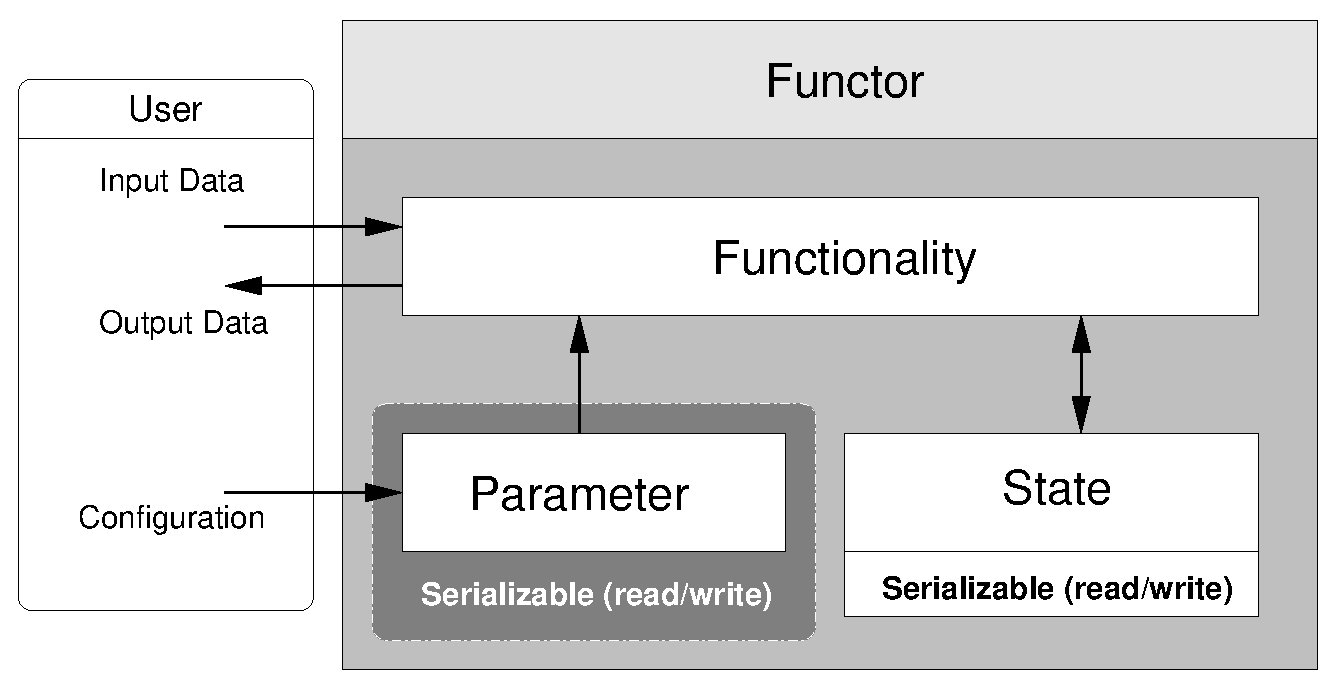
\includegraphics[width=10cm]{fig/functor}
    \caption{Architecture of a functor.  The user can change the behavior of
      the functor through the parameters.  The functor can also have a state,
      that eventually (like the parameters) can also be saved.}
    \label{fig:functor}
  \end{center}
\end{figure}


There are several reasons for an independent parameters class.  You can create
several instances with different value sets and change at once the
functionality of your functor with a simple \code{setParameters()}.  You can
load and save your parameters object in a file, or can give it to a graphical
user interface where the user can choose between several values.

The parameters contain values directly specified by the user and they should
not be modified by the functor.  If a programmer thinks his/her
algorithm must change a parameter, this is just a sign that this parameter
should be copied somewhere else at the beginning of the algorithm, like a
local variable or a state variable (an attribute of the functor class).

An usual question is: why do I need to call the method \code{getParameters()}
to get the parameters instance? would it not be faster if each functor-class
had its own parameters instance that it could use directly?

\begin{figure}[htbp]
  \begin{center}
    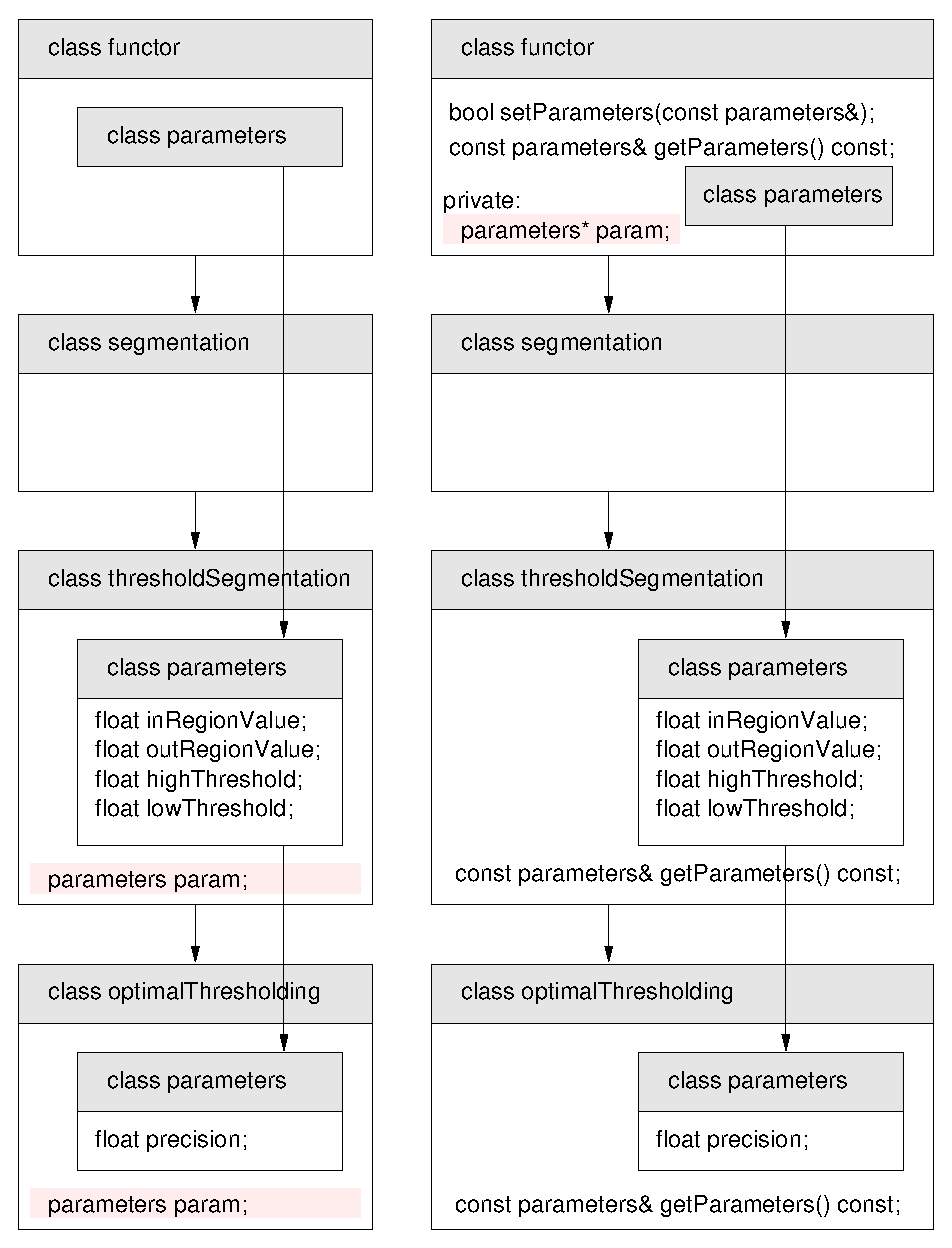
\includegraphics[height=16cm]{fig/paramhier}
    \caption{Example for the functor hierarchy: on the left side the naive way
      with several parameters-class instances (this implies a very inefficient
      memory management).  On the left side the \ltilib\ way with just one
      parameters-class instance.}
    \label{fig:paramhier}
  \end{center} 
\end{figure}

The answer relies partially on memory management issues.  It would be very
expensive if all classes in the functor hierarchy would have their own instance
of the parameters, because all inherited parameter attributes would be present
several times.  With the functor hierarchy shown on the left side of
Fig.~\ref{fig:paramhier}  an instance of the functor
\code{lti::optimalThresholding} would have two parameter objects: the one of
its own with five attributes (\code{precision} and the five attributes of the
parent class) and the parameters-instance of \code{lti::thresholdSegmentation}
with its four attributes.  In other words, the four attributes of the parent
class are present twice!

To avoid this problem, there exist just one instance of the parameters in the
functor class.  Each class casts this instance to the proper parameters type
using the overloaded method \code{getParameters()}.

Another important reason for the use of just one parameters-instance in the
functor class appears when the inherited class calls methods of the parent
classes, the later ones could not see the proper parameters-instance but only
the own one, which could contain other values than those specified by the
user.

The functionality of a functor is always accessed by its methods
\code{apply}.  They expect input data, (usually constant references to objects
like matrices or images), and references to output objects (references to
containers where the result is written).  Functors also provide the so
called \emph{shortcut}-methods that simplify the use of specific
functionality.  For example, to load an image file, the image loaders provide
the shortcut \code{load} that expects the file name and the image where the
result should be left.  Otherwise, you would require to create a parameters
object, set there the filename, give this parameters-instance to the functor,
and at last call the apply method:

{\small
\begin{alltt}
  // an image
  lti::image img;

  // functor to load images in Windows BMP format:
  lti::loadBMP loader;

  // parameters for the loader
  lti::loadBMP::parameters loaderParam;

  // the file to load
  loaderParam.filename = "testimage.bmp";

  // load the image into img
  loader.setParameters(loaderParam);
  loader.apply(img); // load the image!

\end{alltt}
}

It is much easier and comfortable to employ following shortcut:

{\small
\begin{alltt}
   // an image
  lti::image img;

  // functor to load images with Windows BMP format:
  lti::loadBMP loader;

  // load an image
  loader.load("testimage.bmp",img);
    
\end{alltt}
}

All functors must nevertheless provide an interface based on a
\code{parameters}-object and \code{apply}-methods, in order to provide complex
higher-level applications a uniform way to access the functionality of the
functor.

Within the apply methods you can avoid an unnecessary copy of the
parameters-instance getting a constant reference to them, for example:

{\small
\begin{alltt}
/*
 * apply method for myFunctor. Do something on the src vector and
 * leave the result in the dest vector.
 * @param src the input vector
 * @param dest the output vector
 * @return true if successful, false otherwise
 */
 myFunctor::apply(const vector<double>& src, vector<double>& dest) \{
   
   // Get a const reference to the functor parameters
   const parameters\& param = getParameters();

   // use the parameters to do something, assuming you have
   // an attribute called "justCopy" in the parameters
   if (param.justCopy) \{
     dest.copy(src)
   \} else \{
     // do something else ...
   \}

   return true;
 \}
\end{alltt}
}

Please remember, the parameters should never be changed within the
\code{apply}-methods:     

{\small
\begin{alltt}
bool myFunctor::apply(...) \{

  ...

  const parameters& param = getParameters();

  param.justCopy = false;  // is not possible, param is const!
  
  // you should NEVER EVER do something like this:
  const_cast<parameters*>(&param)->justCopy = false;

  // do something like:
  
  // a local copy of the parameters' attribute
  bool justCopy(param.justCopy);

  justCopy = false; // the local copy may be changed!

  ...
\}
\end{alltt}
}

There exist just one \code{getParameters}-method and it returns a
\emph{constant} reference to the parameters-instance, this due to the fact
that the parameters must not be changed by the functor.

As mentioned above, the functor may provide some \emph{shortcuts}
that allow changing specific parameter values.  These methods, of course,
should not be called within the \code{apply} methods.

Besides the parameters, a functor may have a state, where it stores
information irrelevant for the user but necessary for later computations.
An example for a functor with separated state and parameters is the
\code{lti::principalComponents} object.  Here you find a parameter
\code{autoDim} which indicates that another parameter
\code{resultDim} should be detected automatically.  In the \code{apply} method
this last value is not changed.  The computed transformation matrix is part of
the functor state, which can be used later to transform other vectors.  This
matrix is not something that the user can give directly, but can be saved and
loaded with other parts of the functor's state (this is done when you
load or save the whole functor).

All functors with a state relevant for later computations can be saved and
loaded, i.\,e.\ they overload the methods \code{read} and \code{write}.

\section{Input and Output in the \ltilib}

Serializable objects in the \ltilib (\ie\ objects that can be written or read
from disk) never directly use \code{std::fstream} objects.  The main reason is
that we need to provide a way to support different file formats at the same
time.  The desired file format is determined through a so called
\code{lti::ioHandler}.  At this time there are two file formats.  A Lisp-like
one writes or reads ASCII strings in or from a given stream, where
different scopes are delimited with parenthesis.  A binary format 
produces shorter files and is faster to be read or written, but can not be
edited by hand.

A uniform way to load or save \ltilib-objects and internal types (\code{int},
\code{float}, \code{double}, \code{std::string}, etc.) is provided through
four global functions that passes them properly to a given \code{ioHandler}.
These are:

{\small
\begin{alltt}
  bool lti::write(ioHandler& handler, 
                  const T& data);

  bool lti::read(ioHandler& handler,
                 T& data);


  bool lti::write(ioHandler& handler, 
                  const std::string& name,
                  const T& data,
                  const bool complete=true);

  bool lti::read(ioHandler& handler, 
                 const std::string& name,
                 T& data,
                 const bool complete=true);
\end{alltt}
}

The first two functions write or read the contents of an object of type
\code{T} in or from the given \code{ioHandler}.  The third and fourth methods
write the data together with a name that identifies this object.  To read
the data, the given name must match the one used as the data was saved.

With a handler of type \code{lti::lispStreamHandler} following lines
{\small
\begin{alltt}
  lti::write(handler,"a",5);
  lti::write(handler,"b",9);
\end{alltt}
}

produce the following output in the output stream associated with the handler:
{\small
  \begin{alltt}
    (a 5)
    (b 9)
  \end{alltt}
}

The parenthesis around each line can be left out if the fourth parameter of
the functions (\code{complete}) is set to \code{false}.  Note that the default
value for this parameter is \code{true}.

The \code{lti::lispStreamHandler} can find an object using its name:
{\small
\begin{alltt}
  int x,y;
  lti::read(handler,"a",x);
  lti::read(handler,"b",y);
\end{alltt}
}

After these lines it applies \code{x==5} and \code{y==9}.  Some
\code{ioHandler} (for example \code{binaryStreamHandler}) require that the
read order matches the one used when writing.  If this is not true, the read
methods will return \code{false}.  Other \code{ioHandler} (like
\code{lispStreamHandler}) search for the data using the given name as key, so
that you can use a different reading order.  Following lines would also result
in \code{x==5} and \code{y==9}:

{\small
\begin{alltt}
  int x,y;
  lti::read(handler,"b",y);
  lti::read(handler,"a",x);
\end{alltt}
}

The \code{ioHandler} concept makes it possible to define new file formats
\emph{without} requiring to reimplement all read and write methods of the
\ltilib-classes.  Due to the fact that the read and write methods use a
rigorous syntax, it is also relative simple to parse the files.

Please note that the variables used in the previous examples could also have
any other type defined in the \ltilib.   All numerical standard types
(\code{int}, \code{double}, etc.), the Standard Template Library (STL) types 
\code{std::vector}, \code{std::list} and \code{std::map} (if you include the
file ``\code{ltiSTLIoInterface.h}'') and the most \ltilib\ functors,
parameters and data structures can be serialized.

\subsection{Example}

How can I save and load some parameters in my program?

{\small
\begin{alltt}

  // ltilib functors and their parameters
  lti::csPresegmentation segmentor;
  lti::csPresegmentation::parameters segParam;

  lti::orientationFeature orientor;
  lti::orientationFeature orientParam;

  // ... initialize the parameters ...

  // how can we write the parameters in a file named "param.txt"?
  lti::lispStreamHandler handler;  // the stream handler
  std::ofstream out("param.txt");  // the std::fstream used

  // if the output stream is ok, write the data
  if (out) \{
    // the handler have to write the data using the stream "out":
    handler.use(out);
    
    // write the parameters:
    lti::write(handler,"orientParam",orientParam); 
    lti::write(handler,"segmentParam",segParam);
    lti::write(handler,"anInteger",5);
  \}


  // how can we read the data from "param.txt"?
  std::ifstream in("param.txt");

  if (in) \{
    int x;

    handler.use(in);
    
    // read the data
    lti::read(handler,"orientParam",orientParam); 
    lti::read(handler,"segmentParam",segParam);
    lti::read(handler,"anInteger",x);
  \}
\end{alltt}
}

\section{Visualization Classes}

Not everything in an image processing or computer vision library can be
considered as functor.  Examples for this are the so called drawing and
visualization objects.

Drawing objects does not execute one algorithm.  They provide different tools
to draw simple geometric constructs on images or other output media.  To use a
drawing object you need to provide it with your \emph{canvas}, \ie\ you need to
specify the image where you want to draw.  This is done with the method
\code{use}.  After that, you can choose the color you want to use with the
method \code{setColor}.  All lines, circles or points you draw after this,
will be painted using the given color.

Following example draws a circle and a line on a color image:

{\small
\begin{alltt}
  lti::image img(256,256);  // our canvas

  lti::draw<rgbPixel> drawing;  // drawing tool
  
  drawing.use(img);                      // where should "drawing" paint on?
  drawing.setColor(lti::Blue);           // Blue color
  drawing.circle(lti::point(128,128),
              20,true));              // filled circle, radius 20
  drawing.setColor(lti::Red);            // Red color
  drawing.line(10,10,128,128);           // A red line
\end{alltt}
}

Viewer objects do not modify any data, but provide simple ways to
visualize them.  The presentation of the data persists as long as the viewer
object exists.

You can show the previously drawn image with following code:

{\small
\begin{alltt}
  lti::viewer viewer("This is art");  // our viewer object
  viewer.show(canvas);                // show our master piece
  getchar();                          // just wait 
\end{alltt}
}

\section{Classifiers}

Other important object classes that do not fit into the functor paradigm are
the classifiers.  They provide methods to learn from data and to use the
learned information to analyze new data.  There are different interfaces for
the supervised and unsupervised classifiers.  Both types can be categorized
into instance classifiers that learn single vectors (like traditional neural
networks) and sequence classifiers that also considered time aspects (like the
Hidden Markov Models).

In the \ltilib\ all classifiers deliver the results using the same data
structures \code{lti::classifier::outputVector}, so that the processing of
their results does not depend on the specific classifier used.

%%% Local Variables: 
%%% mode: latex
%%% TeX-master: "DevelopersGuide"
%%% End: 
